\section{Numerical Stability Analysis}
\subsection{Method}
\begin{frame}{Principle}
\begin{itemize}
\item Stable direct integration scheme:
\begin{equation*}
\exists h_0 > 0 \hspace{0.5cm}\text{such as} \hspace{0.5cm} \forall h \in [0,h_0]
\end{equation*}  
a finite perturbation of the state vector at $t_n$ gives a non increasing variation of the state vector at a subsequent time $t_{n+j}$.
\item Initial disturbance:
\begin{equation}
\delta X_0 = X_0^\prime - X_0
\end{equation}
\item The non-perturbed solution:
\begin{align}
X_{n+1} &= H X_n + g_{n+1} \\
&= H^2 X_{n-1} + Hg_n + g_{n+1} \\
&\vdots\\
&= H^{n+1}X_0 + \sum^{n+1}_{j=0} H^{n-j+1}g_j
\end{align}
\end{itemize}
\end{frame}

\begin{frame}
\begin{itemize}
\item Perturbed solution:
\begin{equation}
X^\prime_{n+1} = H^{n+1}X_0^\prime + \sum^{n+1}_{j=0} H^{n-j+1}g_j
\end{equation}
\item Effect of initial disturbance at time $t_{n+1}$:
\begin{equation}
\delta X_{n+1} = H^{n+1} \delta X_0
\end{equation}
\item Eigenvalues of amplification matrix $H$ :
\begin{equation}
det(H-\lambda I) = 0
\end{equation}
\item $\lambda_r, x_{(r)}$ associated eigenvalues and eigenvectors.
\end{itemize}
\end{frame}
\begin{frame}
\begin{itemize}
\item Modal expension:
\begin{equation}
\delta X_0 = \sum^{2N}_{s=1} a_s x_{(s)}
\end{equation}
\item Transform the recurrence relation to:
\begin{align}
\delta X_{n+1} &= H^{n+1} \sum^{2N}_{s=1} a_s x_{(s)} \\
&= \sum^{2N}_{s=1} a_s \lambda_s^{n+1} x_{(s)}
\end{align} 
\item Disturbance will be amplified if eigenvalues are higher than unity.
\end{itemize}
\end{frame}

\begin{frame}
\begin{itemize}
\item Equation of motion at time $t_{n}$ and $t_{n+1}$:
\begin{equation}
\begin{cases}
    M  \Ddot{U}^n = -C \Dot{U}^n - K U^n +P_{int}^n \\
    M \Ddot{U}^{n+1} = -C \Dot{U}^{n+1} - K U^{n+1} +P_{int}^{n+1} 
\end{cases}
\end{equation}
\item And the recurrence relationships by Newmark method (it could be another method):
\begin{equation}
\begin{cases}
\dot{U}_{n+1} = \dot{U}_n + (1-\gamma)dt \ddot{U}_n + \gamma dt \ddot{U}_{n+1} \\
U_{n+1} = U_n +dt \dot{U}_n + dt^2 \left(\frac{1}{2}-\beta\right) \ddot{U}_n + dt^2 \beta \ddot{U}_{n+1}
\end{cases}
\end{equation}
\item Check the stability for $h = [0.001, 10]$ by step of $0.001$. 
\end{itemize}
\end{frame}
\subsection{1D stability}
\begin{frame}{1D bar element}
\begin{itemize}
\item \underline{1D bar element :}
\begin{figure}
\centering
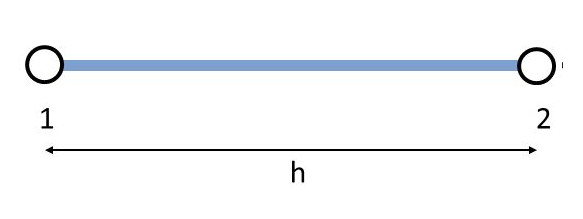
\includegraphics[width=0.5\linewidth]{images/bar-element.jpg}
\end{figure}
\item 4 eigenpairs : corresponding to 2 rigid body motions and traction-elongation modes. 
\end{itemize}
\end{frame}

\begin{frame}{1D bar element: Implicit}
\begin{figure}[ht] 
  \label{ fig7} 
  \begin{minipage}[b]{0.5\linewidth}
    \centering
    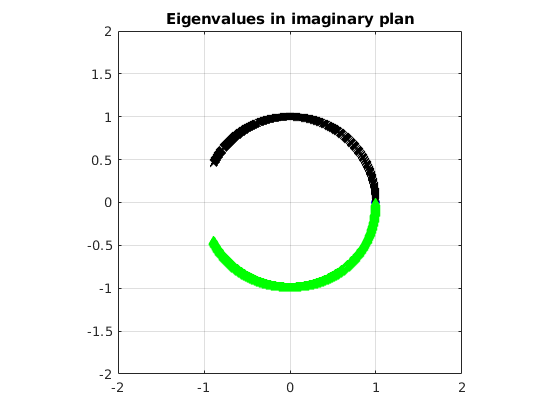
\includegraphics[scale=.35]{images/bar-imp-1.png} \\

  \end{minipage}%%
  \begin{minipage}[b]{0.5\linewidth}
    \centering
    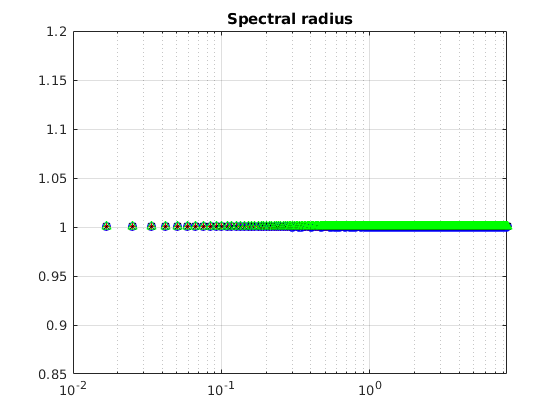
\includegraphics[scale=.35]{images/bar-imp-2.png} \\
  \end{minipage} 
  \begin{minipage}[b]{0.5\linewidth}
    \centering
    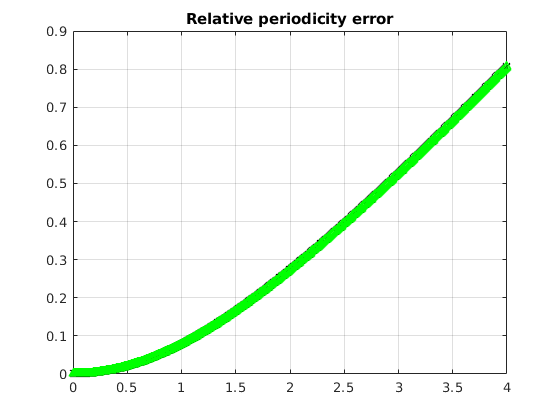
\includegraphics[scale=.35]{images/bar-imp-3.png} \\

  \end{minipage}%% 
  \begin{minipage}[b]{0.5\linewidth}
    \centering
    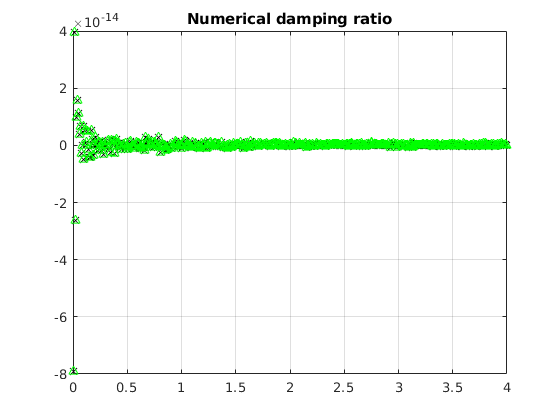
\includegraphics[scale=.35]{images/bar-imp-4.png} \\

  \end{minipage} 
\end{figure}
\end{frame}

\begin{frame}{1D bar element: Explicit}
\begin{figure}[ht] 
  \label{ fig7} 
  \begin{minipage}[b]{0.5\linewidth}
    \centering
    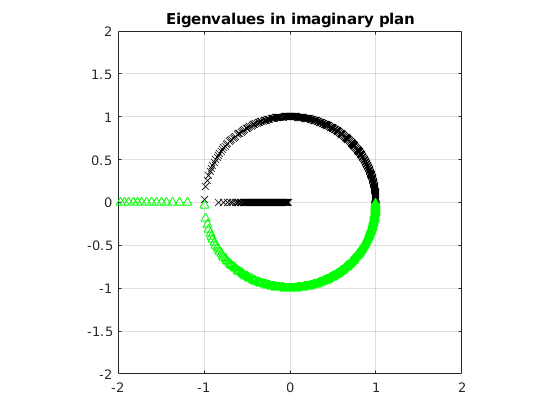
\includegraphics[scale=.35]{images/bar-exp-1.png} \\

  \end{minipage}%%
  \begin{minipage}[b]{0.5\linewidth}
    \centering
    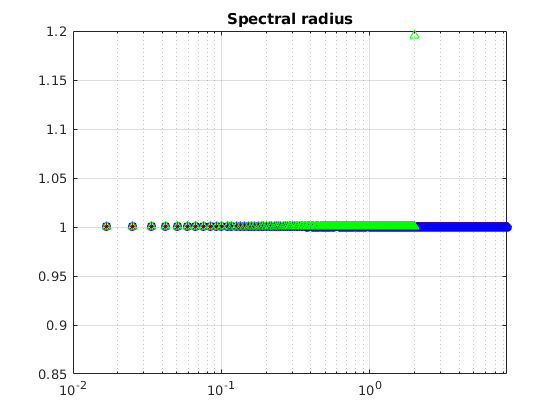
\includegraphics[scale=.35]{images/bar-exp-2.png} \\
  \end{minipage} 
  \begin{minipage}[b]{0.5\linewidth}
    \centering
    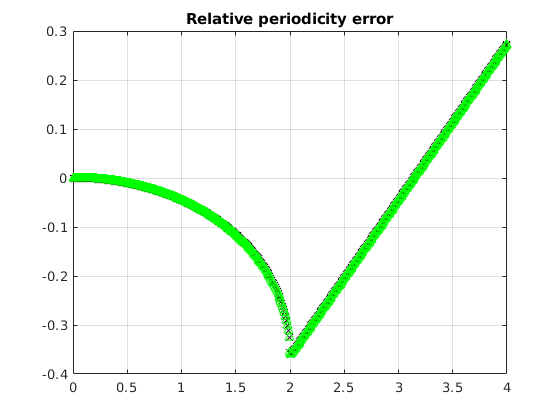
\includegraphics[scale=.35]{images/bar-exp-3.png} \\

  \end{minipage}%% 
  \begin{minipage}[b]{0.5\linewidth}
    \centering
    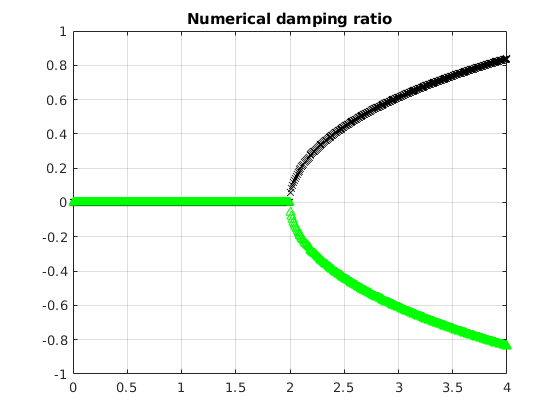
\includegraphics[scale=.35]{images/bar-exp-4.png} \\

  \end{minipage} 
\end{figure}
\end{frame}


\begin{frame}{1D PML bar element}
\begin{itemize}
\item \underline{1D PML bar element :}
\begin{figure}
\centering
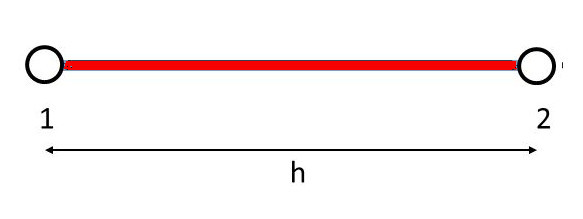
\includegraphics[width=0.5\linewidth]{images/bar-element-pml.jpg}
\end{figure}
\item 6 eigenpairs (depending on the order of numerical quadrature): 2 rigid body motions, traction-elongation and 2 spurious eigenvalues.
\end{itemize}
\end{frame}

\begin{frame}{1D PML bar element: Implicit}
\begin{figure}[ht] 
  \label{ fig7} 
  \begin{minipage}[b]{0.5\linewidth}
    \centering
    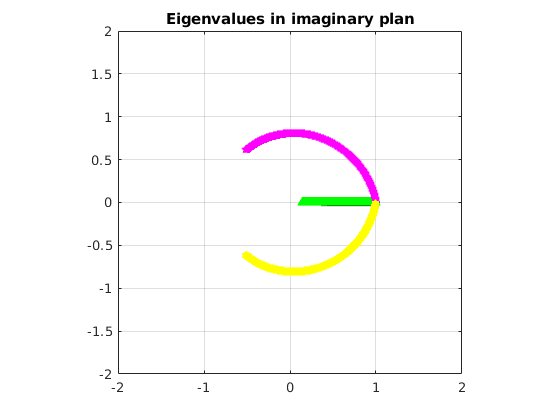
\includegraphics[scale=.35]{images/pml1d-imp-1.png} \\

  \end{minipage}%%
  \begin{minipage}[b]{0.5\linewidth}
    \centering
    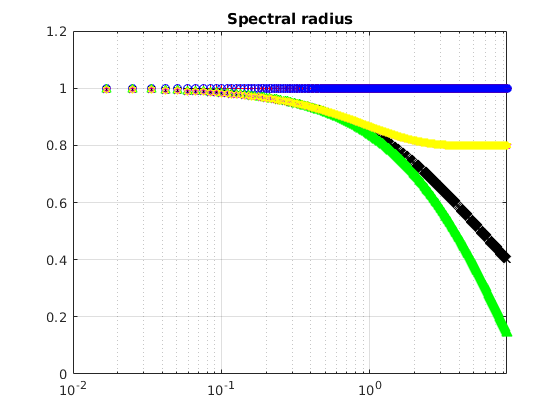
\includegraphics[scale=.35]{images/pml1d-imp-2.png} \\
  \end{minipage} 
  \begin{minipage}[b]{0.5\linewidth}
    \centering
    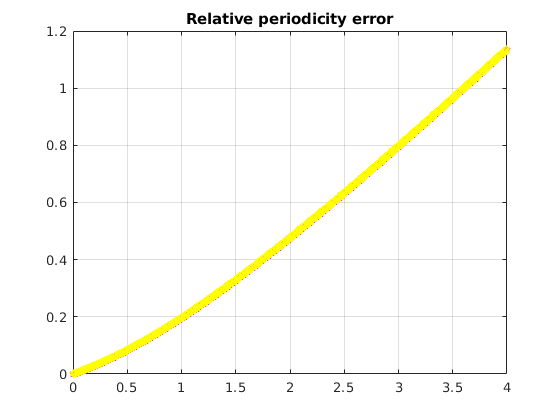
\includegraphics[scale=.35]{images/pml1d-imp-3.png} \\

  \end{minipage}%% 
  \begin{minipage}[b]{0.5\linewidth}
    \centering
    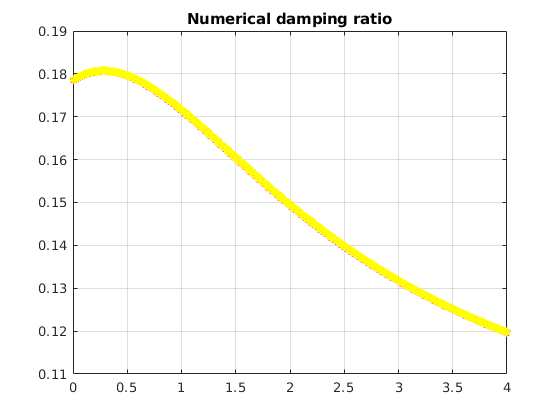
\includegraphics[scale=.35]{images/pml1d-imp-4.png} \\

  \end{minipage} 
\end{figure}
\end{frame}

\begin{frame}{1D PML bar element: Explicit}
\begin{figure}[ht] 
  \label{ fig7} 
  \begin{minipage}[b]{0.5\linewidth}
    \centering
    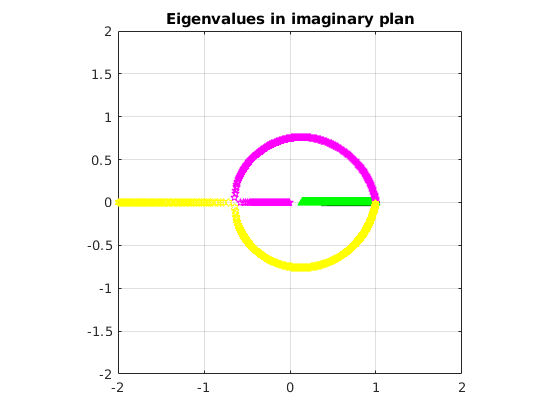
\includegraphics[scale=.35]{images/pml1d-exp-1.png} \\

  \end{minipage}%%
  \begin{minipage}[b]{0.5\linewidth}
    \centering
    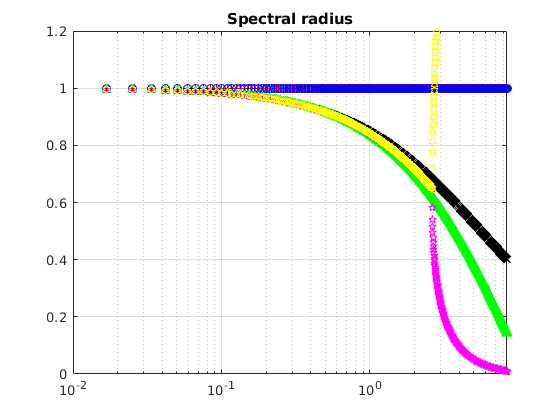
\includegraphics[scale=.35]{images/pml1d-exp-2.png} \\
  \end{minipage} 
  \begin{minipage}[b]{0.5\linewidth}
    \centering
    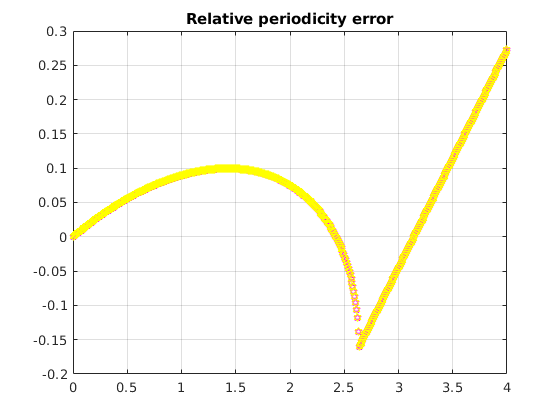
\includegraphics[scale=.35]{images/pml1d-exp-3.png} \\

  \end{minipage}%% 
  \begin{minipage}[b]{0.5\linewidth}
    \centering
    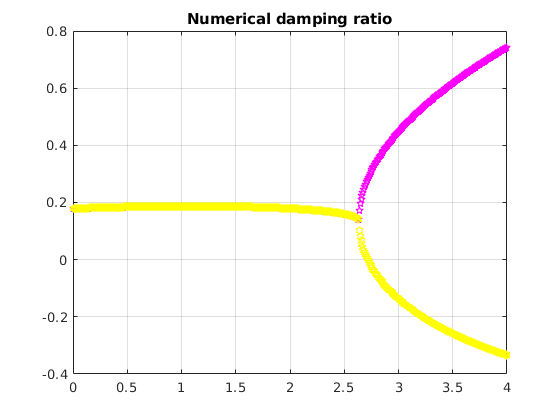
\includegraphics[scale=.35]{images/pml1d-exp-4.png} \\

  \end{minipage} 
\end{figure}
\end{frame}

\subsection{2D stability}
\begin{frame}{2D element stability}
\begin{itemize}
\item \underline{2D linear 4-noded element :}
\begin{figure}
\centering
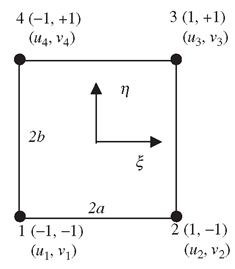
\includegraphics[width=0.4\linewidth]{images/square2d.png}
\end{figure}
\item 8 eigenpairs for the 2D element.
\item At least 52 eigenpairs for the 2D PML element (depending on the order of the numerical quadrature used).
\end{itemize}
\end{frame}

\begin{frame}{2D element: Implicit}
\begin{figure}[ht] 
  \label{ fig7} 
  \begin{minipage}[b]{0.5\linewidth}
    \centering
    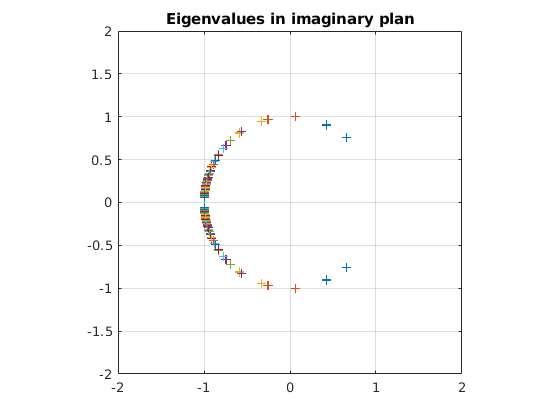
\includegraphics[scale=.35]{images/2D-imp-1.png} \\

  \end{minipage}%%
  \begin{minipage}[b]{0.5\linewidth}
    \centering
    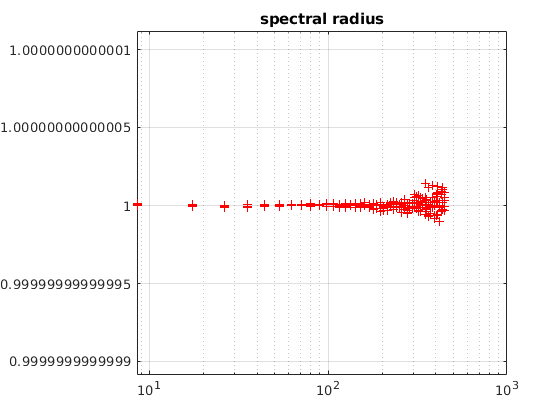
\includegraphics[scale=.35]{images/2D-imp-2.png} \\
  \end{minipage} 
  \begin{minipage}[b]{0.5\linewidth}
    \centering
    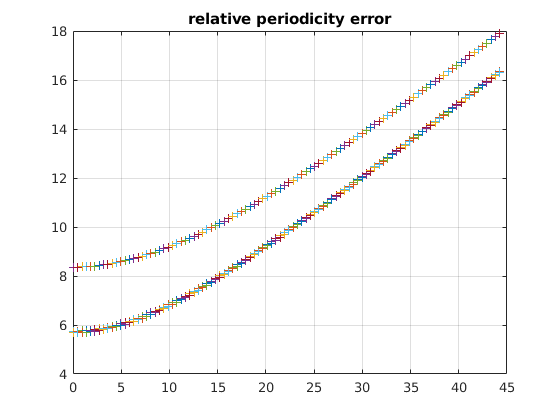
\includegraphics[scale=.35]{images/2D-imp-3.png} \\

  \end{minipage}%% 
  \begin{minipage}[b]{0.5\linewidth}
    \centering
    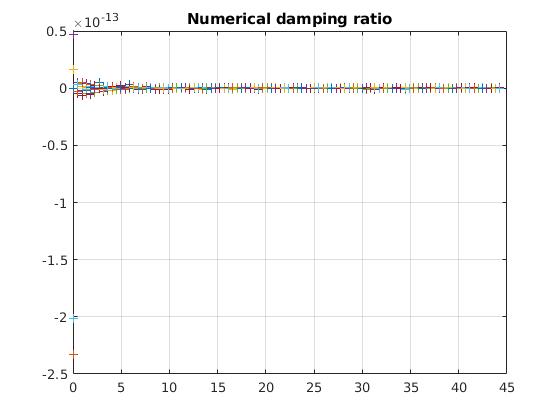
\includegraphics[scale=.35]{images/2D-imp-4.png} \\

  \end{minipage} 
\end{figure}
\end{frame}

\begin{frame}{2D element: Explicit}
\begin{figure}[ht] 
  \label{ fig7} 
  \begin{minipage}[b]{0.5\linewidth}
    \centering
    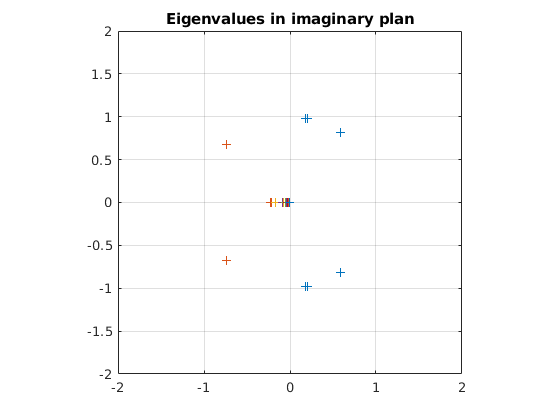
\includegraphics[scale=.35]{images/2D-exp-1.png} \\

  \end{minipage}%%
  \begin{minipage}[b]{0.5\linewidth}
    \centering
    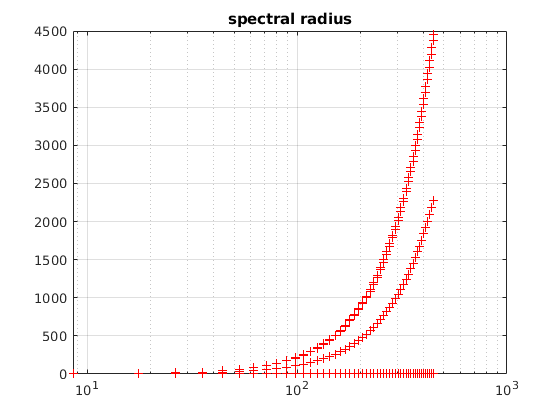
\includegraphics[scale=.35]{images/2D-exp-2.png} \\
  \end{minipage} 
  \begin{minipage}[b]{0.5\linewidth}
    \centering
    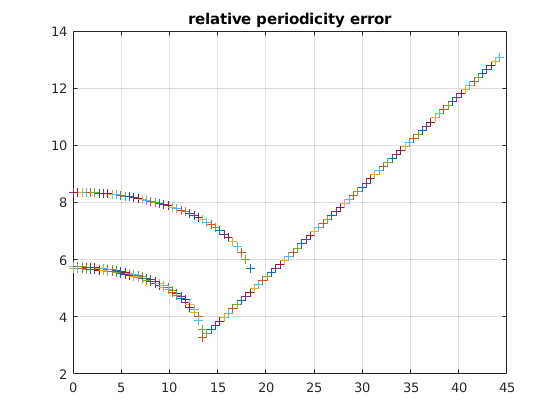
\includegraphics[scale=.35]{images/2D-exp-3.png} \\
  \end{minipage}%% 
  \begin{minipage}[b]{0.5\linewidth}
    \centering
    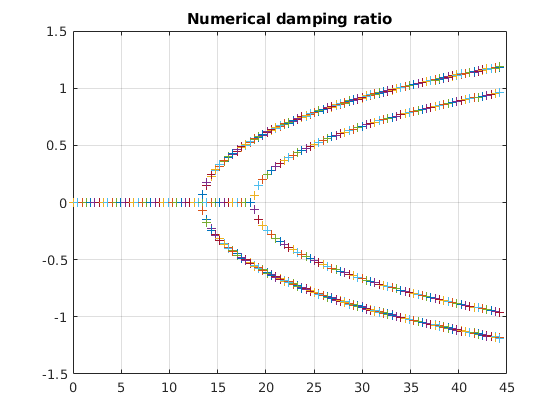
\includegraphics[scale=.35]{images/2D-exp-4.png} \\
  \end{minipage} 
\end{figure}
\end{frame}

\begin{frame}{2D PML element: Implicit}
\begin{figure}[ht] 
  \label{ fig7} 
  \begin{minipage}[b]{0.5\linewidth}
    \centering
    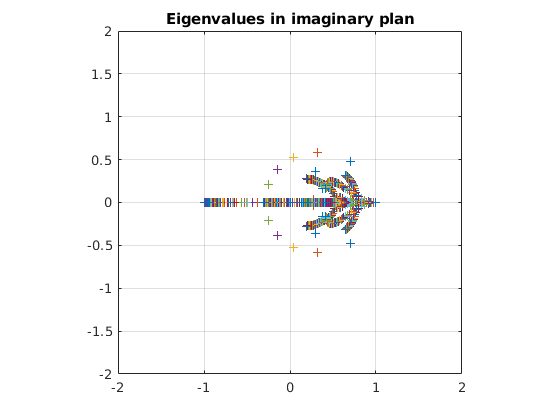
\includegraphics[scale=.4]{images/2Dpml-imp-1.png} \\

  \end{minipage}%%
  \begin{minipage}[b]{0.5\linewidth}
    \centering
    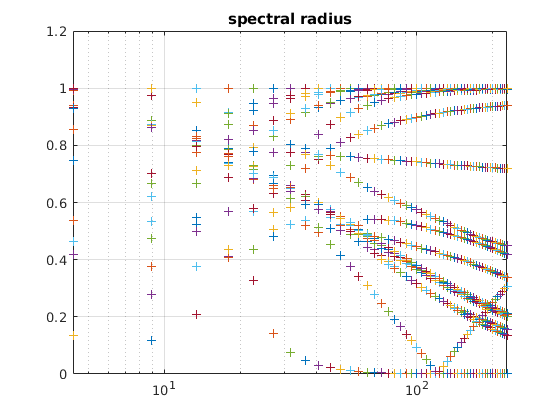
\includegraphics[scale=.4]{images/2Dpml-imp-2.png} \\
  \end{minipage} 

\end{figure}
\end{frame}

\begin{frame}{2D PML element: Explicit}
\begin{figure}[ht] 
  \label{ fig7} 
  \begin{minipage}[b]{0.5\linewidth}
    \centering
    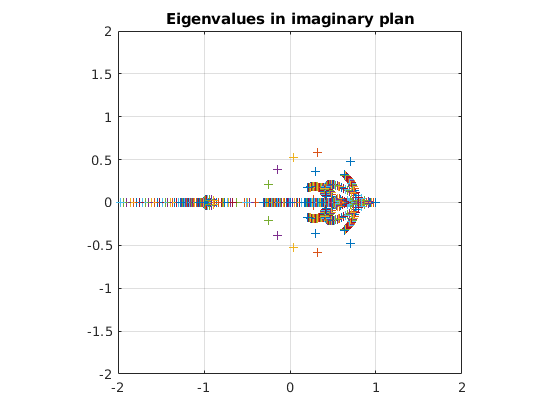
\includegraphics[scale=.4]{images/2Dpml-exp-1.png} \\

  \end{minipage}%%
  \begin{minipage}[b]{0.5\linewidth}
    \centering
    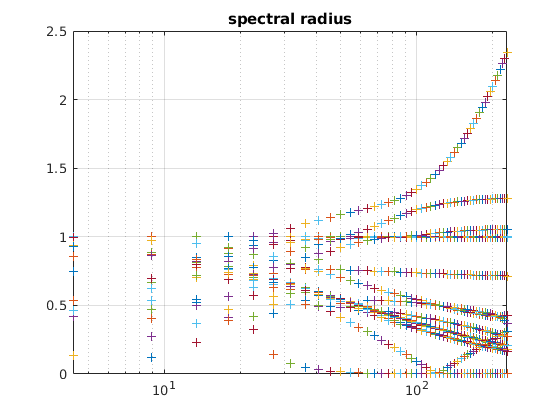
\includegraphics[scale=.4]{images/2Dpml-exp-2.png} \\
  \end{minipage} 

\end{figure}
\end{frame}